\subsection{Indflydelse af basrefleksens placering}
I dette afsnit vil der blive set på hvordan placeringen af basrefleksen kommer til, at spille en rolle i kabinettets samlede frekvenskarakteristik. Ligesom før ønskes der variabel-kontrol og derfor vil der kun blive målt på betydningen, når en lang basrefleks placeres forskellige steder på højtalerkabinettet.

Der er ikke blevet gennemgået nogen dybdegående teori der forklarer frekvensresponsets afhængighed af basrefleksen - alligevel ønsker gruppen at lave nogle empiriske undersøgelser.

Ved måling af betydningen af basrefleksens placering var det vigtigt, at ingen af basrefleksrørene var blokeret på den ene eller anden facon. Dette var især vigtigt for undersiderefleksen idet højtalerkabinettet måtte placeres på ben for ikke at blokere denne.

Nedenfor ses måleresultaterne, når basrefleksen bliver placeret forskellige steder i kabinettet men der måles på membranen.
\begin{figure}[H]
	\centering
	\vspace{-12pt}
	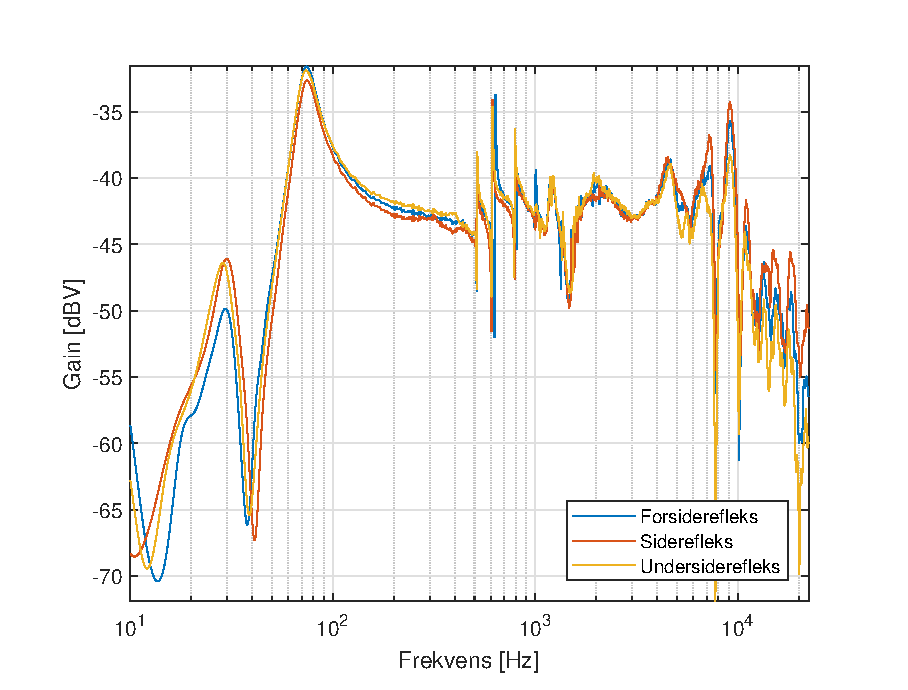
\includegraphics[width=\textwidth]{Billeder/Grafer/BasrefleksPlacementClose}
	\caption{Betydning af basrefleksens placering (målt på membran)}
\end{figure}

Det ses at der ikke forekommer den helt store forskel på membranens karakteristik alt efter hvor basrefleksen placeres. Dette er dog også at forvente, idet koblingen mellem basrefleks og membran ikke er ligefrem.

Det ses dog, at når basrefleksen placeres på forsiden, så vil frekvenskarakteristikken være omtrent \SI{4}{\decibel} lavere ved \SI{30}{\hertz} end når den placeres andre steder.

\newpage
Ligesom før så måles der nu på basrefleksens egen frekvenskarakteristik, når den bliver placeret forskellige steder på kabinettet. Det forventes her, at forskellen i frekvensresponserne vil være større end ved membranens eget frekvensrespons. Resultaterne er vist nedenfor.
\begin{figure}[H]
	\centering
	\vspace{-12pt}
	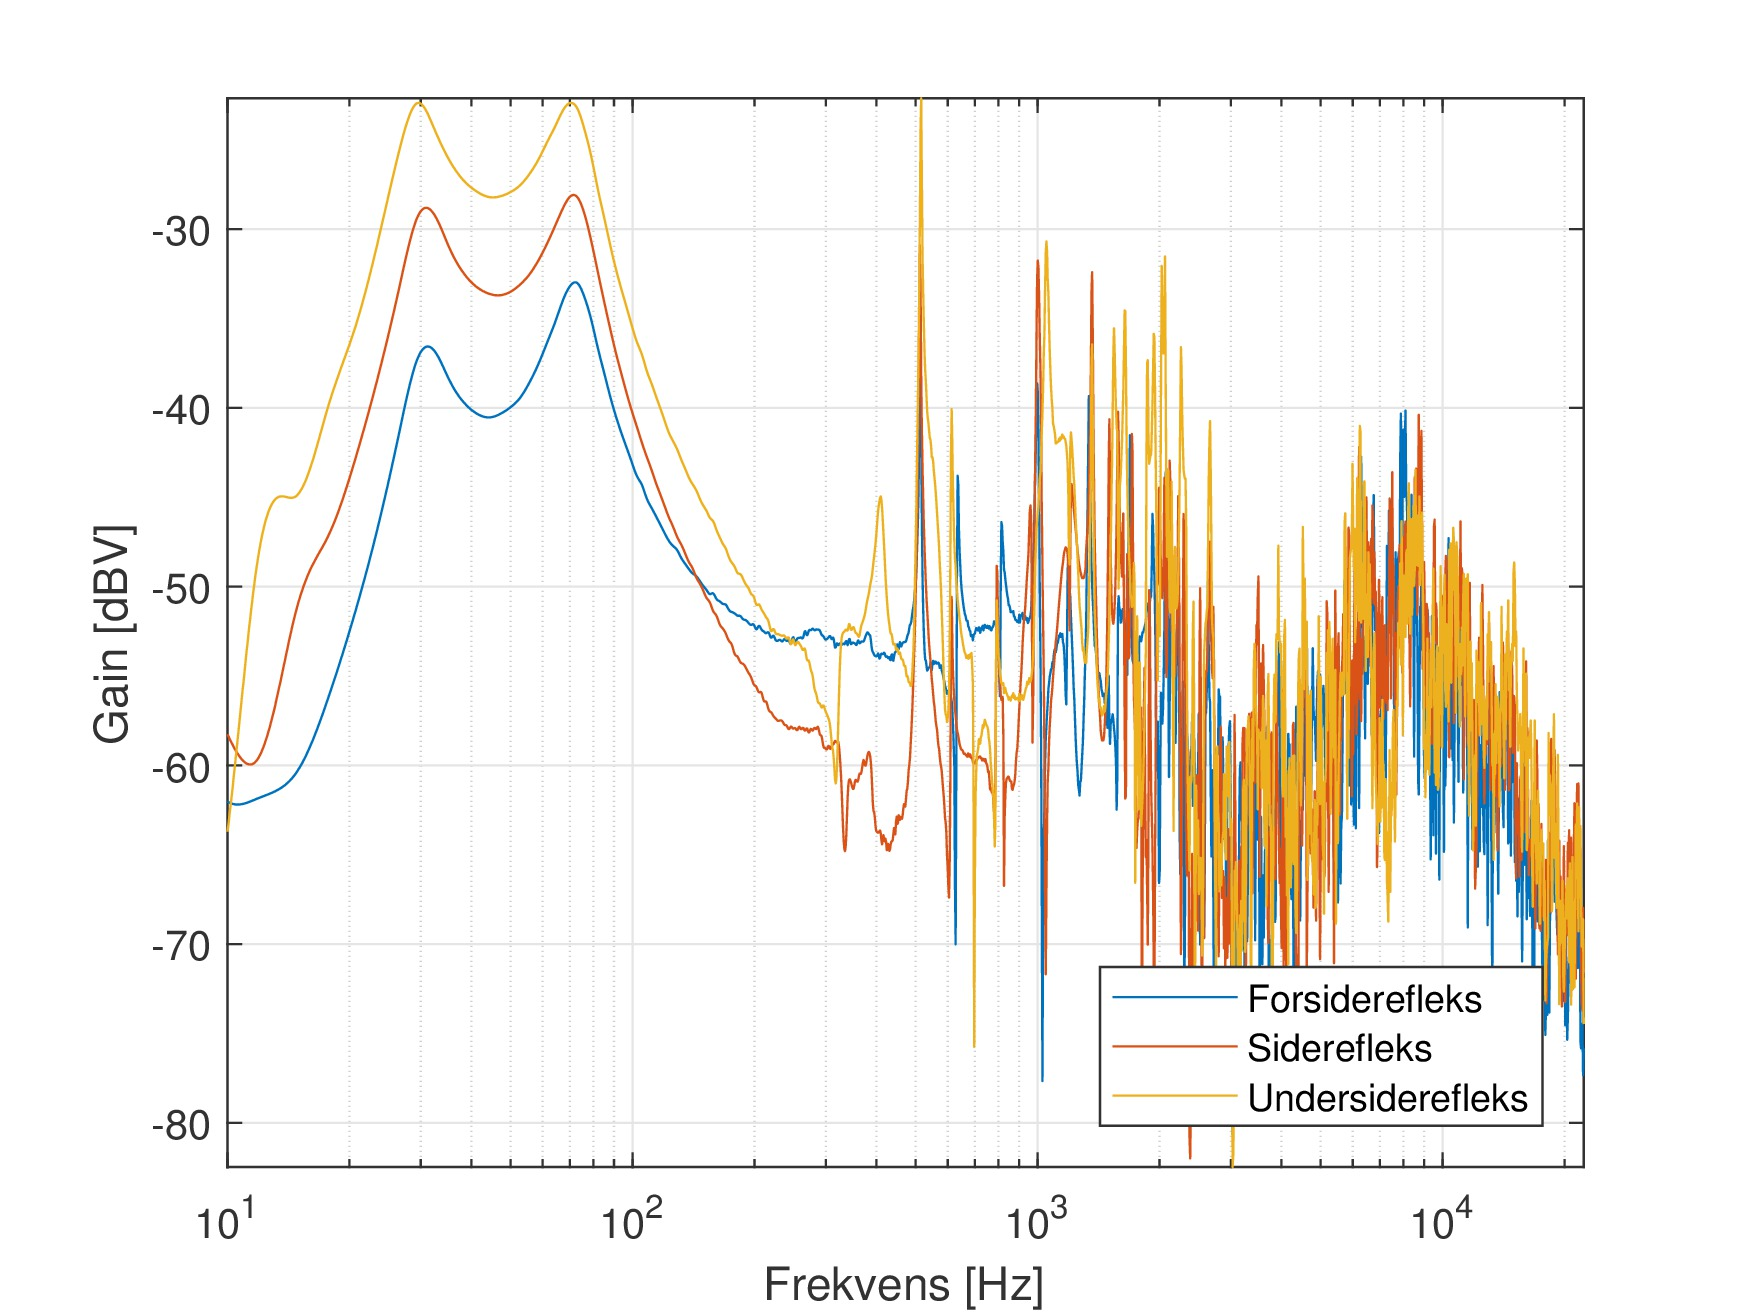
\includegraphics[width=\textwidth]{Billeder/Grafer/BasrefleksPlacementTube}
	\caption{Betydning af basrefleksens placering (målt på basrefleks)}
\end{figure}

Som forventet så er der ikke den store forskel i frekvensresponsernes udseende, men nogle placeringer af basrefleksen vil åbenbart foresage en større forstærkning end andre frekvenser. Det ses at en forsiderefleks giver den laveste forstærkning, en siderefleks giver en middel forstærkning og en undersiderefleks giver den største forstærkning. Dette havde vi ikke umiddelbart forventet.

\newpage
Til sidst blev der målt på hvordan en eventuel lytter vil opfatte højtalerens lyd. Dette blev gjort ved, at placere CLIO-mikrofonen i en afstand på \SI{1}{\meter} fra højtalermembranen.

Det er klart at siden lytteren står direkte foran membranen, så vil han/hun ikke kunne lytte til basrefleksens fulde udbytte, når basrefleksen er placeret på siden eller i bunden af kabinettet. Alligevel har gruppen antaget at dette vil være den mest naturlige position for en lytter.
\begin{figure}[H]
	\centering
	\vspace{-12pt}
	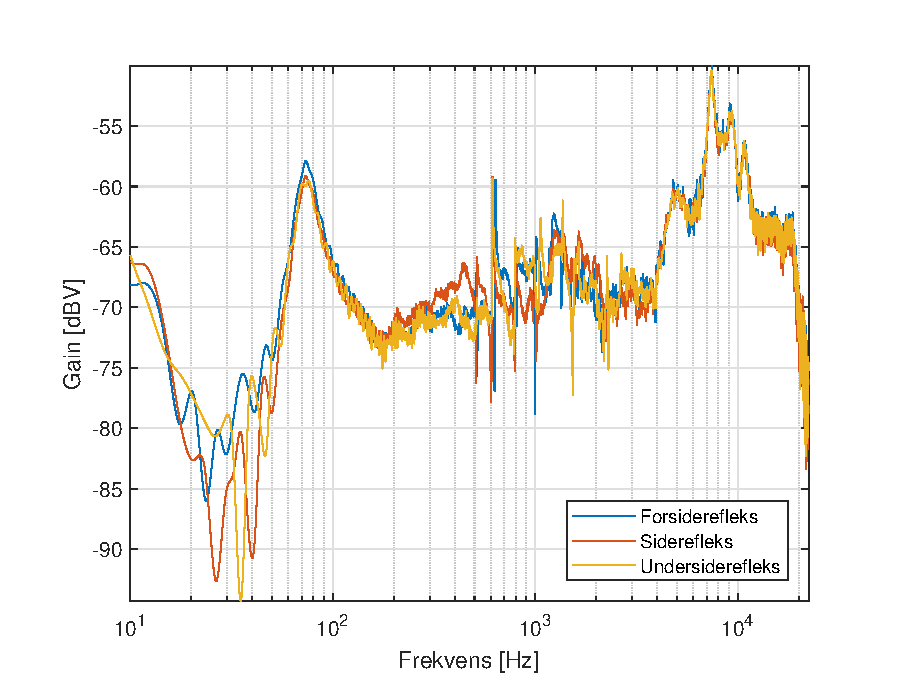
\includegraphics[width=\textwidth]{Billeder/Grafer/BasrefleksPlacementFar}
	\caption{Betydning af basrefleksens placering (målt i lytteafstand)}
\end{figure}

Det ses hurtigt, at højtalerens målte frekvenskarakteristik ved de høje frekvenser ikke afhænger særlig meget af basrefleksens placering. Der forekommer dog afvigelser i de lave frekvenser (\SI{20}{\hertz} til \SI{50}{\hertz}) hvor det ses, at en forsiderefleks giver den største forstærkning i dette område. Dette er altså en smule mod de forventninger gruppen havde fra basrefleksens egen frekvenskarakteristik hvor en undersiderefleks virkede bedst.

Grunden til dette fænomen må være, at lytteren er placeret foran membranen og at han/hun kræver reflektioner for, at kunne opleve udbyttet fra basrefleksen placeret på siden eller undersiden af kabinettet. De refleksioner som lytteren modtager vil dog være meget dæmpet på grund af det lyddøde rums egenskaber og derfor oplever lytteren ikke disse bidrag.